
% !TeX root = master.tex

\hypertarget{tuning-reference}{%
\section{Tuning reference}\label{tuning-reference}}

This file documents the gain scheduling rules in \texttt{tuning.js}. All
variable names refer to \texttt{KALMAN\_TUNING} so the plots stay tied
to the actual configuration. Plots are generated by
\texttt{scripts/plot\_tuning.py}.

\hypertarget{process-noise-vs-boat-length-acceleration-variance}{%
\subsection{Process noise vs boat length (acceleration
variance)}\label{process-noise-vs-boat-length-acceleration-variance}}

We scale the base acceleration variance by boat length so longer boats
respond more slowly. For lengths shorter than the anchor, we do not
increase the base value.

\[
q = \text{baseQ} \left(\frac{L_0}{\max(L_0, L)}\right)^2
\]

Variables:
\begin{itemize}
\tightlist
\item
  \texttt{KALMAN\_TUNING.processNoise.baseAccelerationVariance} =
  \(\text{baseQ}\)
\item
  \texttt{KALMAN\_TUNING.processNoise.baseBoatLengthMeters} = \(L_0\)
\end{itemize}

\begin{figure}
\centering
\includegraphics{./plots/gain-q-length.pdf}
\caption{Process noise vs boat length}
\end{figure}

\hypertarget{speed-scale-from-recent-max-speed}{%
\subsection{Speed scale from recent max
speed}\label{speed-scale-from-recent-max-speed}}

The process noise is further scaled by recent max speed (not
instantaneous speed). We use the maximum speed over a recent window to
capture the boat's potential to accelerate even if it is currently slow.

\[
\text{speedScale} = \frac{\max(v^*_{\text{kn}}, v_{\min})}{v_{\text{anchor}}}
\]

Variables:
\begin{itemize}
\tightlist
\item
  \texttt{KALMAN\_TUNING.processNoise.speedScale.minKnots} = \(v_{\min}\)
\item
  \texttt{KALMAN\_TUNING.processNoise.speedScale.anchorKnots} =
  \(v_{\text{anchor}}\)
\item
  \texttt{KALMAN\_TUNING.processNoise.speedScale.recentMaxSpeedWindowSeconds}
  defines the window used to compute \(v^*\)
\end{itemize}

\begin{figure}
\centering
\includegraphics{./plots/gain-speed-scale.pdf}
\caption{Speed-based gain scale}
\end{figure}

\hypertarget{imu-gravity-low-pass-vs-boat-length}{%
\subsection{IMU gravity low-pass vs boat
length}\label{imu-gravity-low-pass-vs-boat-length}}

The gravity estimate is low-pass filtered so the down axis stays stable
in waves. We scale the low-pass factor by boat length: larger boats get
a slower response.

\[
\alpha = \text{clamp}\left(\alpha_0 \sqrt{\frac{L_0}{\max(L_0, L)}},\; \alpha_{\min},\; \alpha_{\max}\right)
\]

Variables:
\begin{itemize}
\tightlist
\item
  \texttt{KALMAN\_TUNING.imu.gravityLowPass.baseAlpha} = \(\alpha_0\)
\item
  \texttt{KALMAN\_TUNING.imu.gravityLowPass.baseBoatLengthMeters} = \(L_0\)
\item
  \texttt{KALMAN\_TUNING.imu.gravityLowPass.minAlpha} = \(\alpha_{\min}\)
\item
  \texttt{KALMAN\_TUNING.imu.gravityLowPass.maxAlpha} = \(\alpha_{\max}\)
\end{itemize}

\begin{figure}
\centering
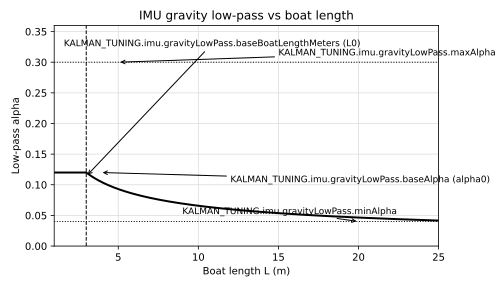
\includegraphics{./plots/gain-gravity-alpha.pdf}
\caption{IMU gravity low-pass vs boat length}
\end{figure}

\hypertarget{process-noise-anisotropy-forward-vs-lateral}{%
\subsection{Process noise anisotropy (forward vs
lateral)}\label{process-noise-anisotropy-forward-vs-lateral}}

Boats change speed much more easily along their heading than sideways.
We encode that by scaling the lateral acceleration variance as a fixed
fraction of the forward variance:

\[
q_{\text{lateral}} = \rho\,q_{\text{forward}}
\]

Variables:
\begin{itemize}
\tightlist
\item
  \texttt{KALMAN\_TUNING.imu.lateralVarianceRatio} = \(\rho\)
\end{itemize}
